\documentclass[conference]{IEEEtran}
% EECR official IEEEtran conference format. Reference-reduction revision 2026-11-18.
\IEEEoverridecommandlockouts
\usepackage{cite}
\usepackage{amsmath,amssymb,amsfonts}
\usepackage{algorithmic}
\usepackage{graphicx}
% Keep floats after their source and within their main section. Subsection
% boundaries remain flexible to avoid short columns and large empty spaces.
\usepackage{flafter}
\usepackage[section]{placeins}
\usepackage{balance}
\usepackage{textcomp}
\usepackage[table]{xcolor}
\definecolor{methodblue}{HTML}{2376AC}
\usepackage{url}
\usepackage[hidelinks]{hyperref}
\def\BibTeX{{\rm B\kern-.05em{\sc i\kern-.025em b}\kern-.08em
    T\kern-.1667em\lower.7ex\hbox{E}\kern-.125emX}}

\title{Engineering Minimum-Cost Reach-Avoid Control for Quadruped Navigation}

\author{
  \IEEEauthorblockN{Haoyang Cao}
  \IEEEauthorblockA{\textit{Institute of Software,}\\
  \textit{Chinese Academy of Sciences}\\
  \textit{University of the Chinese}\\
  \textit{Academy of Sciences}\\
  Beijing, China\\
  caohaoyang24@mails.ucas.ac.cn}
  \and
  \IEEEauthorblockN{Yuhua Guo}
  \IEEEauthorblockA{\textit{Space Star Technology Co., Ltd,}\\
  \textit{China Academy of Space Technology}\\
  \textit{State Key Laboratory of Space}\\
  \textit{Information System and Integrated}\\
  \textit{Application, Beijing Institute of}\\
  \textit{Satellite Information Engineering}\\
  Beijing, China\\
  guoyh@radi.ac.cn}
  \and
  \IEEEauthorblockN{Bai Xue}
  \IEEEauthorblockA{\textit{Key Laboratory of}\\
  \textit{System Software}\\
  \textit{Institute of Software,}\\
  \textit{Chinese Academy of Sciences}\\
  Beijing, China\\
  xuebai@ios.ac.cn}
}
% Jingduo Pan was removed from this version at the user's request.
% The remaining author order follows the archived CoRL submission. Haoyang Cao's
% publication-name spelling is corroborated by Bai Xue's team homepage.
% Yuhua Guo's two affiliations follow the author-provided reference images.
% Their shared Beijing address is listed once after both affiliations.
% All authors' Beijing, China locations are confirmed by the user.
% The corresponding author still requires confirmation; do not infer it.

\begin{document}
% Avoid stretching inter-float and heading glue to force equal column bottoms.
\raggedbottom
\maketitle

\begin{abstract}
The deployment of minimum-cost reach-avoid control on a physical quadruped robot is investigated. The challenges of coupled locomotion--navigation learning and model--execution mismatch are addressed through hierarchical control and two data-calibrated margins. Locomotion stabilization is separated from high-level navigation learning by a pretrained, frozen velocity tracker. Before high-level learning, nominal budget accounting is corrected by the cost margin, and the unsafe set is expanded by the geometric margin. Across three navigation scenarios, a success rate of 73.3\% and a budget violation rate of 9.0\% are obtained with the resulting calibrated minimum-cost reach-avoid (CaMRA) system, compared with 70.7\% and 14.0\% for uncalibrated RC-PPO. The distinct roles and deployment limits of these corrections are examined through ablation, held-out calibration, and physical-robot studies. An execution-calibrated pipeline is established to connect nominal minimum-cost reach-avoid planning with quadruped closed-loop execution.
\end{abstract}

\begin{IEEEkeywords}
quadruped navigation, reach-avoid control, safe robot learning
\end{IEEEkeywords}

\section{Introduction}
Quadruped robots are increasingly used for inspection, exploration, and service
tasks in environments where a navigation policy must do more than reach a target.
The robot must remain collision-free throughout each maneuver while avoiding
unnecessary motion and energy expenditure. These requirements are coupled in
cluttered scenes: a short route may pass close to obstacles, whereas a safer route
may consume more time and actuation. Treating safety and efficiency as independent
reward terms therefore makes the desired trade-off depend on hand-tuned weights.
Minimum-cost reach-avoid (MCRA) control provides a more direct task description by
requiring goal reachability and trajectory-wide avoidance while minimizing a
cumulative cost~\cite{bansal2017}.\footnote{The CaMRA implementation
is publicly available at \url{https://github.com/haoyangc2001/NaVILA_CaMRA}.}

Practical MCRA learning has been enabled by Reachability-Constrained Proximal
Policy Optimization (RC-PPO)~\cite{so2024}.
Within RC-PPO, the state is augmented with a safety indicator and remaining budget,
a reachability value function and budget-conditioned policy are learned, and
the least feasible initial budget is then sought. Safety and cost feasibility in
quadruped navigation are represented jointly through these components.

Deploying this formulation on a physical quadruped requires connecting navigation
decisions to joint-level motion. With direct joint commands, the policy must learn
balance and gait coordination together with collision-free goal reaching. Although
falls, excessive body tilt, and obstacle collisions can be encoded as unsafe
states, these constraints alone do not fully specify coordinated and smooth
locomotion. During early training, informative navigation rollouts may be
interrupted by unstable motion, hindering the learning of route selection and
cost optimization. A low-level velocity tracker is therefore pretrained
to address balance, gait coordination, and action smoothness, and is frozen before
high-level learning. Navigation is then learned through a fixed velocity-command
interface using RC-PPO.

Although the low-level controller improves locomotion stability and attenuates
disturbances, residual mismatch remains between the nominal model and actual
execution. The same velocity-command sequence may incur additional cost or produce
path deviations, causing the high-level planner to underestimate budget
consumption or overestimate obstacle clearance. To address these discrepancies,
the low-level controller is frozen, and paired nominal and executed
rollouts are collected with identical initial conditions and command sequences. A
cost margin $\alpha$ and a geometric safety margin $\delta$ are then calibrated from the
empirical distributions of cost overruns and path deviations, respectively. The
running cost used in budget updates is increased by the cost margin to account for
execution-induced overhead, while the unsafe set is expanded by the geometric margin to
accommodate path deviations. High-level policy learning and budget search are
subsequently performed using the calibrated model, and the resulting policy is
deployed through the same frozen controller.

An ideal MCRA learner is connected to physical closed-loop execution through the
calibrated minimum-cost reach-avoid (CaMRA) deployment pipeline. No strict
stochastic safety guarantee or extension of RC-PPO's deterministic theory to general
stochastic systems is claimed; the scope is limited to empirical robustness under
the execution distribution used to calibrate the margins. The pipeline is evaluated
through controlled mismatch studies, component-wise ablations, sensitivity tests,
and a quantitative physical-robot deployment study. The experiments are designed to
quantify execution mismatch through this fixed interface, assess whether
$\alpha$ and $\delta$ address different failure modes, and evaluate how the
complete system behaves on hardware.

The main contributions are summarized as follows:
\begin{enumerate}
\item A hierarchical framework is developed for quadruped minimum-cost reach-avoid
      navigation. Locomotion stabilization is separated from navigation learning
      through a pretrained, frozen velocity tracker, which provides a consistent
      interface for calibration and deployment.
\item Two execution margins are calibrated from paired nominal and executed
      trajectories. Budget accounting and unsafe-set geometry are corrected
      separately to incorporate execution mismatch into high-level learning and
      budget selection.
\item The roles of both margins and their deployment trade-offs are examined
      through navigation comparisons, ablations, held-out calibration tests, and
      physical-robot evaluation.
\end{enumerate}

\section{Related Work}
\subsection{Minimum-Cost Reach-Avoid Learning}
In reach-avoid reinforcement learning, reaching a target and avoiding an unsafe
set are treated as trajectory-level requirements rather than competing reward terms
\cite{bansal2017,hsu2021}. This formulation is extended to minimum-cost
reach-avoid control in RC-PPO through state augmentation with a safety indicator
and remaining budget, budget-conditioned policy and reachability-critic learning,
and a search for the least feasible initial budget~\cite{so2024}. This formulation
is adopted as the algorithmic foundation for connecting nominal MCRA decisions
to quadruped execution.

\subsection{Safe Quadruped Navigation}
Quadruped navigation in challenging environments is supported by
learning-based locomotion controllers. Robust locomotion on natural terrain
using proprioceptive feedback was demonstrated by Lee et al.~\cite{lee2020}.
At the navigation level, a policy
was trained by Jin et al.~\cite{jin2023resilient} to issue velocity commands to an
existing locomotion controller and respond to perception failures using
locomotion-level observations. In contrast, a joint-level agile policy was
developed by He et al.~\cite{he2024abs}, with reach-avoid-guided switching to a
recovery policy for collision avoidance. Visual navigation and reusable motor
skills are connected through hierarchical policies in prior
work~\cite{jain2021pixels}. At the local-planning level, smooth,
collision-free paths are learned from depth observations using differentiable
cost maps in iPlanner~\cite{yang2023iplanner}. A hierarchical architecture is
adopted here, with a frozen velocity tracker handling
locomotion stabilization and a high-level MCRA policy addressing goal reaching,
obstacle avoidance, and cumulative cost.

\subsection{Robust Deployment under Model--Execution Mismatch}
Model uncertainty is addressed through domain and dynamics randomization by
broadening the training distribution~\cite{tobin2017,tan2018simreal},
or through robust reinforcement learning by optimizing performance across uncertain
dynamics~\cite{wang2021}. The need for dynamics randomization
also depends on the control design and deployment conditions~\cite{xie2021randomization}.
In chance-constrained and risk-aware planning, uncertainty is instead incorporated
into planning constraints or risk measures~\cite{theurkauf2023,fan2021step}.
For example, STEP estimates stochastic traversability for risk-aware off-road
planning~\cite{fan2021step}.
Planning--tracking mismatch is bounded through reachability analysis in
FaSTrack~\cite{herbert2017fastrack}, while model-based planning and learned tracking
are combined in DTC to improve accuracy and robustness~\cite{jenelten2024dtc}.
Here, residual execution errors under a fixed velocity interface are addressed:
empirical quantiles of paired nominal and executed rollout errors are
used to calibrate cost and geometric margins for MCRA learning and deployment.

\section{Problem Formulation}
\label{sec:problem_setup}
\subsection{MCRA and RC-PPO Recap}
The navigation layer is modeled as a discrete-time process with state $x_t\in
\mathcal{X}$, high-level velocity command $u_t\in\mathcal{U}^{\mathrm{high}}$,
transition kernel $P$, running cost $c$, and initial-state distribution $\rho_0$.
The MCRA objective is to reach a goal set $\mathcal{G}$, avoid an unsafe set
$\mathcal{F}$ at every step, and minimize the accumulated cost up to a freely
chosen terminal time $T$:
\begin{equation}
\min_{\pi,T}\quad \sum_{t=0}^{T-1}c(x_t,\pi(x_t))
\label{eq:mcra_objective}
\end{equation}
\begin{equation}
\begin{gathered}
\mathrm{s.t.}\quad x_T\in\mathcal{G},\\
x_t\notin\mathcal{F}\ \forall t\leq T,\\
x_{t+1}\sim P(\cdot\mid x_t,\pi(x_t)).
\end{gathered}
\label{eq:mcra_constraints}
\end{equation}
The sets are represented using signed functions $g$ and $h$ as
$\mathcal{G}=\{x:g(x)\leq0\}$ and $\mathcal{F}=\{x:h(x)>0\}$. Following
RC-PPO~\cite{so2024}, the state is augmented to $\hat{x}_t=(x_t,y_t,z_t)$,
where $y_t\in\{-1,1\}$ records whether the unsafe set has been entered, and $z_t$
denotes the remaining cost budget, initialized at $z_0$. The shifted indicator is
$I_{b\in\mathcal{B}}=+1$ when $b\in\mathcal{B}$ and $-1$ otherwise; thus
$y_{t+1}=\max\{I_{x_{t+1}\in\mathcal{F}},y_t\}$ and
$z_{t+1}=z_t-c(x_t,u_t)$. The augmented goal function is
\begin{equation}
\hat{g}(x,y,z)=\max\{g(x),Cy,-z\},
\label{eq:augmented_goal}
\end{equation}
where $C>0$ is an arbitrary safety-violation constant. RC-PPO notes that a
practical choice is $C=\max_{x\in\mathcal{X}}g(x)$~\cite{so2024}. Reaching the
zero sublevel set of $\hat{g}$ therefore encodes goal reaching, trajectory-wide
avoidance, and the upper-bound property $z_0\geq\sum_t c_t$. The reachability critic,
budget-conditioned actor, and two-phase minimum-budget search from RC-PPO are
adopted as the high-level decision backbone.

\subsection{Quadruped Closed-Loop Execution}
On hardware, $u_t$ is a desired body velocity that is realized by a locomotion
controller. Let $P_{\mathrm{cl}}$ denote the closed-loop transition induced by
this controller. The nominal model used for high-level learning is
$x_{t+1}=\bar f_{\mathrm{cl}}(x_t,u_t)$, while the executed transition is sampled
from $P_{\mathrm{cl}}(\cdot\mid x_t,u_t)$. The difference is the deployment gap
addressed by CaMRA. For a paired nominal/executed rollout, the relative
cost overrun and a trajectory-deviation statistic are defined as
\begin{equation}
\varepsilon_c=\frac{J_{\mathrm{exec}}-J_{\mathrm{nom}}}{J_{\mathrm{nom}}},
\qquad
\varepsilon_d=d(\tau_{\mathrm{exec}},\tau_{\mathrm{nom}}),
\label{eq:execution_errors}
\end{equation}
Here $J$ is a nonnegative navigation proxy cost in arbitrary units (a.u.),
not measured electrical energy. The same command program and time window are
used for both rollouts in a pair;
$d$ is the maximum planar distance between their time-aligned positions.

\subsection{Deployment Objective and Scope}
The deployment objective is to retain the RC-PPO MCRA semantics while accounting
for the measured distribution of $(\varepsilon_c,\varepsilon_d)$. These quantities
are treated as empirical descriptions of the nominal-to-execution gap rather
than as a new stochastic reachability model. This gap is addressed through a
fixed velocity interface, paired rollout data, and calibrated margins for
high-level learning and deployment.

\section{Execution-Calibrated CaMRA}
% TASK-010--TASK-012: interface, mismatch dataset, alpha/delta calibration,
% robustified RC-PPO learning and deployment algorithm.
\subsection{System Overview}
The CaMRA architecture is shown in Fig.~\ref{fig:system_overview}. A high-level
MCRA navigation policy is coupled with a pretrained, frozen low-level velocity
tracker. System development is divided into two stages. First, the tracker is
trained and frozen, and paired nominal and executed rollouts are collected to calibrate the
cost margin $\alpha$ and geometric margin $\delta$. Second, these margins are
incorporated into RC-PPO-based high-level learning and initial-budget selection.
During deployment, body-velocity commands are generated by the navigation policy
and converted into joint commands by the frozen tracker for closed-loop execution.

\begin{figure}[!htbp]
\centering
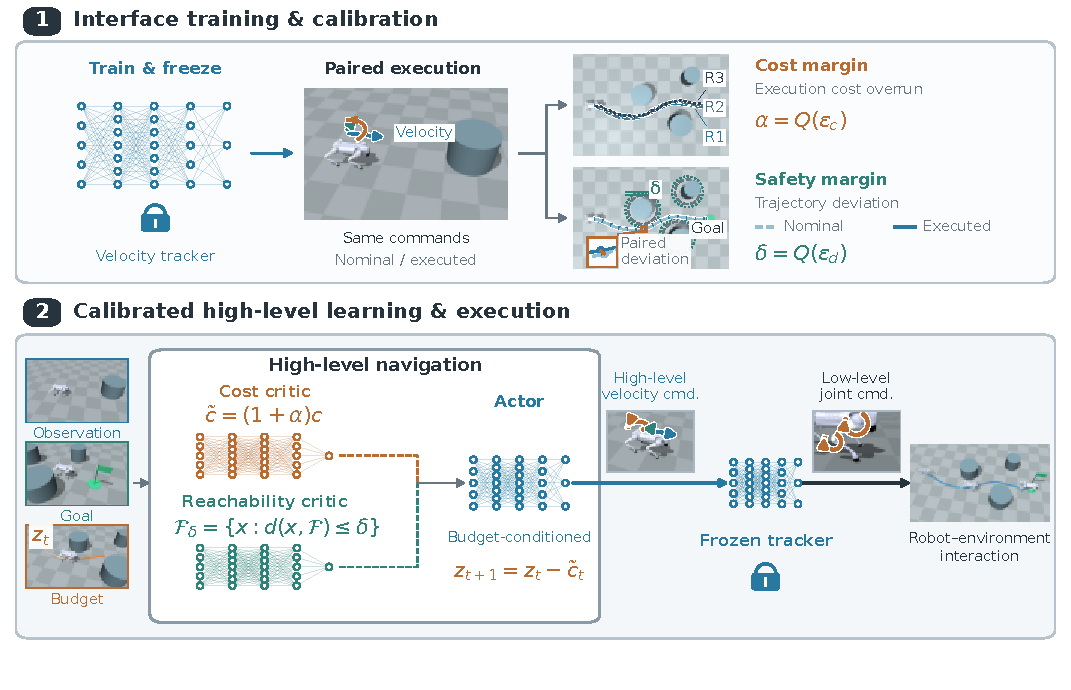
\includegraphics[width=\columnwidth]{../../images/1114/deployment_calibration_overview.pdf}
\caption{CaMRA architecture. In Stage 1, a frozen velocity interface is established
and execution margins are calibrated. In Stage 2, the margins are incorporated into
high-level navigation learning and budget selection, with the same tracker retained for execution.
Scenes and paths are schematic; successive robot states are represented by ghost poses.}
\label{fig:system_overview}
\end{figure}

\subsection{Hierarchical Control with a Frozen Velocity Interface}
With direct joint-level MCRA learning, stable locomotion would have to be learned
alongside goal reaching, obstacle avoidance, and cost reduction.
Although falls and excessive body tilt can be represented as unsafe states,
avoiding these states alone provides limited guidance for learning coordinated and
smooth locomotion. Frequent loss of balance during early training can also
interrupt navigation exploration. A hierarchical architecture is therefore adopted
to separate locomotion stabilization from high-level reach-avoid decisions.

The low-level tracker is pretrained using PPO and domain randomization to track
velocity commands while maintaining balance, gait coordination, and action
smoothness. Proprioceptive observations and body-velocity commands
$u_t=[v_x^*,v_y^*,\omega_z^*]^\top$ are mapped to joint commands. Execution
disturbances are attenuated through closed-loop feedback within the trained
command domain. The tracker is then frozen before mismatch calibration and
high-level learning, so the execution interface is not altered by subsequent
low-level parameter updates. The high-level policy is consequently trained to
issue velocity commands rather than coordinate joint actions directly.

The nominal map $\bar f_{\mathrm{cl}}$ abstracts this interface by integrating
commanded body velocities over each high-level decision interval under ideal
tracking. Deviations from this abstraction can arise from contact variation,
friction, actuation latency, and state-estimation errors. The same frozen
tracker and command domain are retained for calibration, high-level learning, and
deployment, providing a consistent basis for measuring residual mismatch and
calibrating the execution margins.

\subsection{Execution-Mismatch Calibration}
\label{sec:execution_calibration}
To convert execution mismatch into cost and safety margins, paired nominal and
executed rollouts are collected through the frozen velocity interface. For each
pair, identical initial states, maps, goals, and high-level command sequences are
used for the nominal rollout and its perturbed execution. For a rollout of length $T$, let
$J_{\rm nom}=\sum_{t=0}^{T-1}c(x_t^{\rm nom},u_t)$ and
$J_{\rm exec}=\sum_{t=0}^{T-1}c(x_t^{\rm exec},u_t)$. Disjoint rollout sets are
used for calibration and independent evaluation, with evaluation data excluded
from margin selection.

For $J_{\rm nom}>0$, the relative cost overrun $\varepsilon_c$ is computed from
the paired cumulative costs using the definition in Section~\ref{sec:problem_setup}.
Geometric deviation is measured as the maximum planar distance between
time-aligned base positions,
\begin{equation}
\varepsilon_d=\max_{0\leq t\leq T} \left\|p_t^{\rm exec}-p_t^{\rm nom}\right\|_2,
\label{eq:max_planar_deviation}
\end{equation}
where $p_t$ is the base position.

The two errors are calibrated separately to account for their effects on different
MCRA constraints. For quantile levels $p_c$ and $p_d$, the margins are set to
\begin{equation}
\alpha=Q_{p_c}(\varepsilon_c),\qquad
\delta=Q_{p_d}(\varepsilon_d),
\label{eq:calibration_margins}
\end{equation}
where $Q_p$ denotes the empirical $p$-quantile of the calibration samples. The
calibrated running cost is
$\tilde c(x_t,u_t)=(1+\alpha)c(x_t,u_t)$, so the remaining budget evolves as
$z_{t+1}=z_t-\tilde c(x_t,u_t)$. The unsafe set is dilated to
$\mathcal{F}_\delta=\{x:d(x,\mathcal{F})\leq\delta\}$. Both margins are determined
before high-level learning and are held fixed, with empirical coverage dependent on the
execution conditions represented in the calibration data.

\subsection{Robust MCRA Learning and Deployment}
A budget-conditioned navigation policy is trained using the calibrated cost and
expanded unsafe set, and an initial budget is selected for execution through the
frozen velocity interface. The margins are incorporated into learning, so navigation
decisions are optimized under the corrected cost and safety conditions.

In Phase I, budget updates are computed using the calibrated running cost $\tilde c$,
while the safety indicator and augmented goal are determined from the expanded
unsafe set $\mathcal{F}_\delta$. A stochastic actor
$\pi_\theta(u\mid o,y,z)$ and two critics are used: goal reaching and safety
are evaluated by $V_h$, while corrected cumulative cost is estimated by $V_c$
over the same stopping horizon. With cost normalized by the scene-specific
reference budget $z_{\rm ref}>0$, the combined residual is
\begin{equation}
W=\max\{V_h,V_c-z/z_{\rm ref}\}.
\label{eq:combined_residual}
\end{equation}
The actor is optimized to reduce this residual. Accordingly, cost targets and
budget updates are modified through $\alpha$, whereas reachability targets are
modified through $\delta$ via the safety indicator.

In Phase II, a deterministic deployment policy is obtained from the actor's mean
action, and the critics are refitted with the actor fixed. Candidate initial
budgets are evaluated under the calibrated model, and the smallest tested budget
satisfying the prescribed goal-reaching, collision, and budget-violation criteria
is selected.

During deployment, navigation observations and the remaining budget are supplied
to the policy. The resulting body-velocity commands are executed through the
frozen tracker. The calibrated cost used to update the remaining budget is
obtained from a parallel nominal rollout driven by the same commands.

\section{Experiments}
% Evaluation: overall performance, calibration mechanisms, budget sensitivity,
% execution perturbations, and hardware deployment.
\subsection{Experimental Setup and Evaluation Protocol}
\label{sec:experimental_setup}
Navigation performance, execution-error calibration, margin contributions and
sensitivity, budget selection, robustness to execution disturbances, and physical
deployment are evaluated. High-level decisions made through the velocity interface are
assessed in the planar navigation benchmark, while quadruped execution is examined
in the hardware study.

The navigation benchmark comprises moderately cluttered, narrow-passage, and
densely obstructed maps, each spanning $8\times8$ m. Test maps, navigation
observations, command limits, and the frozen velocity tracker are shared across
methods, with matched training interaction budgets and network widths. The
high-level decision interval is 0.2 s, and the episode horizon is 30 s. Each method
is evaluated using three policies trained with different random seeds. With
100 trials per policy and scenario, 300 trials are obtained per scenario and
900 overall. Separate rollout sets are used for calibration, training, budget
selection, and final evaluation.

Five metrics are reported: success rate (SR), mean executed cost (Cost), physical
collision rate (CR), budget violation rate (BVR), and mean per-trial minimum
clearance (MC). Success requires collision-free goal reaching before timeout;
budget compliance is assessed separately. Collision and clearance are measured
against a common physical robot footprint. Cost and MC are computed over all
trials up to goal reaching, collision, or timeout; evaluation continues after
the budget is exceeded. The reference budgets
$z_{\rm ref}$ are 120, 140, and 190 a.u. for the moderately cluttered,
narrow-passage, and densely obstructed scenarios, respectively. The normalized
initial budget $z_0/z_{\rm ref}$ expresses the initial budget relative to the
corresponding reference value. Equally weighted means across scenarios are
reported in the tables at $z_0/z_{\rm ref}=1$. Scenario-level intervals describe
test-case variability conditional on the trained policies.

The baselines comprise uncalibrated RC-PPO, reach-avoid learning (RA), reward-based
proximal policy optimization (PPO), and a constrained PPO implementation (CPPO).
The same frozen velocity tracker is used for all methods. For uncalibrated RC-PPO,
both execution margins are set to zero. RA retains goal reaching and obstacle
avoidance but omits cost minimization and the budget input. For PPO and CPPO,
the collision penalty is weighted by $\beta_L=1$ or $\beta_H=5$, representing
lower and higher penalty weights, respectively. CPPO additionally imposes the
expected cumulative-cost constraint $\mathbb{E}[J/z_{\rm ref}]\leq1$.

\subsection{Overall Navigation Performance}
\label{sec:overall_performance}
The complete pipeline is compared with the baselines in Table~\ref{tab:main_results},
and the same five metrics are reported by scenario in Fig.~\ref{fig:metrics_draft}.
Compared with uncalibrated RC-PPO, mean SR is increased from 70.7\% to
73.3\%, mean executed cost is reduced from 91.7 to 88.3 a.u., and BVR is lowered from
14.0\% to 9.0\% with CaMRA; CR remains similar (15.7\% versus 15.0\%). Lower CR
and greater clearance are obtained with RA and CPPO$_{\beta_L}$, at the expense of
lower SR and higher cost and BVR. A joint success--safety--cost trade-off is thus observed.

\begin{table}[!htbp]
\caption{Equal-scene mean performance at $z_0/z_{\rm ref}=1$.
Cost is interpreted jointly with SR.}
\label{tab:main_results}
\centering
\small
\setlength{\tabcolsep}{3pt}
\renewcommand{\arraystretch}{1.12}
\begin{tabular}{@{}lccccc@{}}
\hline
Method & \shortstack{SR\\(\%) $\uparrow$} & Cost & \shortstack{CR\\(\%) $\downarrow$} & \shortstack{BVR\\(\%) $\downarrow$} & \shortstack{MC\\(m) $\uparrow$}\\
\hline
\rowcolor{methodblue!9}
\textbf{CaMRA} & \textbf{73.3} & \textbf{88.3} & 15.0 & \textbf{9.0} & 0.31\\
RC-PPO & 70.7 & 91.7 & 15.7 & 14.0 & 0.30\\
RA & 60.0 & 104.0 & 13.0 & 20.0 & 0.34\\
PPO$_{\beta_L}$ & 67.7 & 99.7 & 23.0 & 20.7 & 0.20\\
PPO$_{\beta_H}$ & 42.3 & 117.0 & 29.0 & 27.0 & 0.16\\
CPPO$_{\beta_L}$ & 37.7 & 124.7 & \textbf{12.3} & 22.3 & \textbf{0.36}\\
CPPO$_{\beta_H}$ & 69.7 & 105.7 & 18.3 & 17.0 & 0.26\\
\hline
\end{tabular}
\end{table}

\begin{figure}[!htbp]
\centering
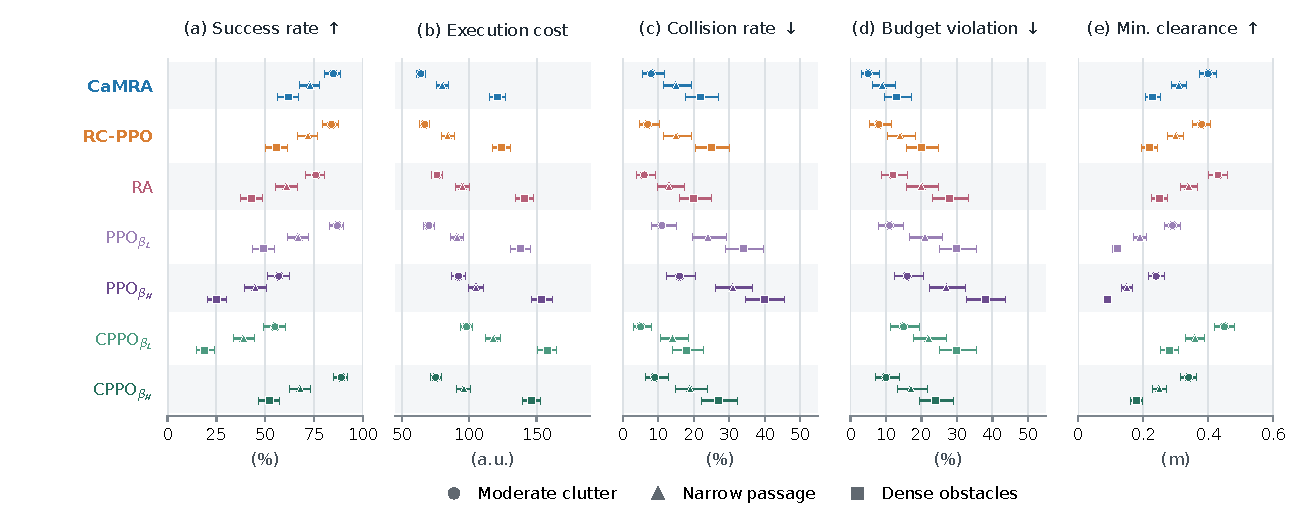
\includegraphics[width=\columnwidth]{../../images/1114/metrics_comparison.pdf}
\caption{Scenario-level SR, Cost, CR, BVR, and MC at the common reference budget.
Scenarios and methods are distinguished by markers and colors, respectively.
Points show the computed metric values; horizontal bars show the corresponding
95\% intervals conditional on the three trained policies ($n=300$ per method and scene). Equal-scene means
are reported in Table~\ref{tab:main_results}.}
\label{fig:metrics_draft}
\end{figure}

Navigation behavior in one paired example is illustrated in
Fig.~\ref{fig:trajectory_sync}. With the geometric margin $\delta$, a slightly
longer, more costly route with greater obstacle clearance is followed with CaMRA.
Obstacle passages are marked in the synchronized curves of clearance, executed
cost, and tracking error. The role of $\alpha$ in budget accounting is illustrated
by the corrected nominal charge. The common budget is satisfied by both methods,
illustrating a safety--cost trade-off. The same proxy cost definition is used in
this separate diagnostic case, which is excluded from Table~\ref{tab:main_results}.

\begin{figure}[!htbp]
\centering
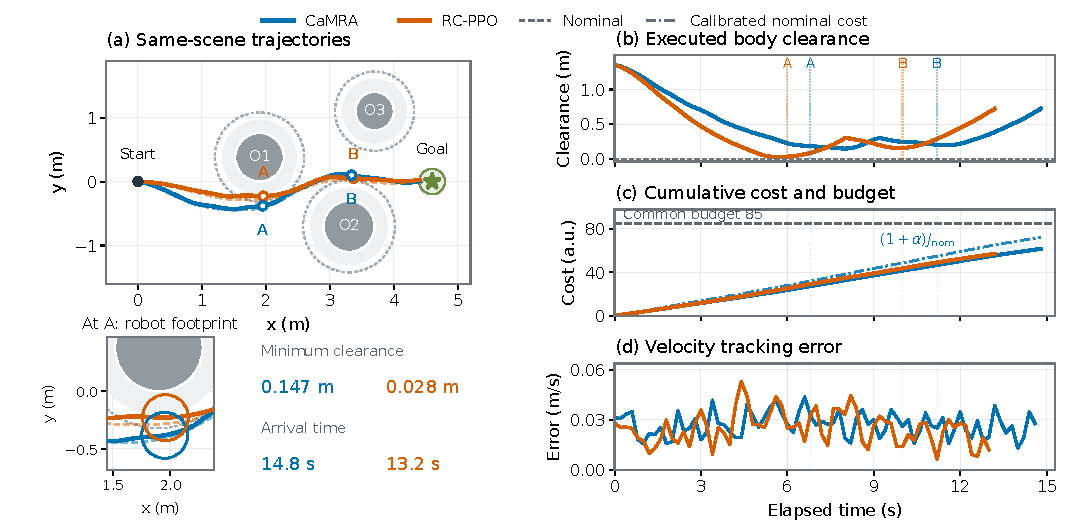
\includegraphics[width=\columnwidth]{../../images/1114/trajectory_sync.pdf}
\caption{Same-scene trajectories and synchronized diagnostics for CaMRA (blue)
and RC-PPO (orange), with a common initial budget of 85 a.u.
(a) Executed (solid) and nominal (dashed) paths, with $\delta=0.12$ m.
(b) Physical clearance. (c) Cumulative costs, budget, and corrected charge
$(1+\alpha)J_{\rm nom}$, with $\alpha=0.18$. (d) Linear-velocity tracking error.
Each method's obstacle passages are marked by A/B; traces are truncated at the
respective terminations.}
\label{fig:trajectory_sync}
\end{figure}

\subsection{Execution-Error Calibration and Margin Analysis}
\label{sec:mismatch_analysis}
Execution mismatch is summarized in Fig.~\ref{fig:margin_calibration} using 800
calibration and 400 held-out paired rollouts. In the calibration set, the medians
are $0.09$ for relative cost overrun and
$0.06$ m for maximum planar position deviation; $\alpha=0.18$ and $\delta=0.12$ m
are set to the respective 90th percentiles. With these margins fixed, held-out
coverage is $353/400$
($88.25\%$) for cost and $346/400$ ($86.50\%$) for position. These marginal
coverages are used to assess the error allowances in budget accounting and obstacle
inflation; joint held-out coverage is $336/400$ ($84.0\%$). Neither marginal nor
joint error coverage is a navigation success probability.

\begin{figure}[!htbp]
\centering
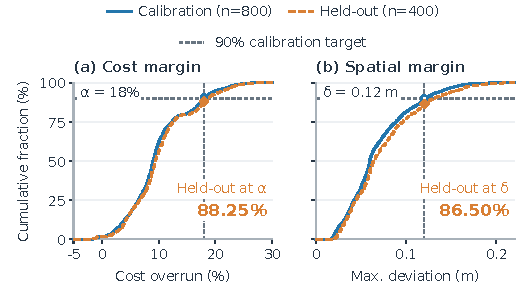
\includegraphics[width=\columnwidth]{../../images/1114/margin_calibration.pdf}
\caption{Execution-error calibration and held-out assessment.
Calibration and held-out empirical CDFs are shown as blue solid and orange dashed
curves. The calibration 90th percentiles and 90\% target are marked by vertical
and horizontal lines, respectively. Coverage at the fixed thresholds, including
ties, is indicated by circles and diamonds.}
\label{fig:margin_calibration}
\end{figure}

The contributions of the two execution margins are examined in
Table~\ref{tab:ablation_draft}, with the same frozen velocity tracker retained in
all variants. For the single-margin ablations, either $\alpha=0$ or $\delta=0$
is imposed, while the other margin is retained at its calibrated value. With both
margins set to zero, the uncalibrated RC-PPO baseline is recovered.
These comparisons are visualized in
Fig.~\ref{fig:ablation_margins}. Without $\alpha$, BVR is increased by
13.4 percentage points; without $\delta$, CR is increased by 11.3 percentage
points and clearance is reduced.

\begin{table}[!htbp]
\caption{Margin ablation with the same frozen tracker and reference budget as
Table~\ref{tab:main_results}.
Cost is interpreted jointly with SR.}
\label{tab:ablation_draft}
\centering
\small
\setlength{\tabcolsep}{3pt}
\renewcommand{\arraystretch}{1.12}
\begin{tabular}{@{}lccccc@{}}
\hline
Variant & \shortstack{SR\\(\%) $\uparrow$} & Cost & \shortstack{CR\\(\%) $\downarrow$} & \shortstack{BVR\\(\%) $\downarrow$} & \shortstack{MC\\(m) $\uparrow$}\\
\hline
\rowcolor{methodblue!9}
\textbf{CaMRA} & \textbf{73.3} & 88.3 & \textbf{15.0} & \textbf{9.0} & \textbf{0.31}\\
w/o both (RC-PPO) & 70.7 & 91.7 & 15.7 & 14.0 & 0.30\\
w/o $\alpha$ & 67.2 & 80.6 & 19.8 & 22.4 & 0.29\\
w/o $\delta$ & 64.8 & \textbf{77.2} & 26.3 & 13.8 & 0.19\\
\hline
\end{tabular}
\end{table}

The CaMRA and RC-PPO results from Table~\ref{tab:main_results} are reused for
the full and zero-margin rows. Each single-margin variant is trained separately
with the corresponding margin removed during both learning and evaluation.
The effects are non-additive, and lower cost can be associated with more failed
trials or shorter trajectories. Cost must therefore be interpreted jointly with
success rate.

\begin{figure}[!htbp]
\centering
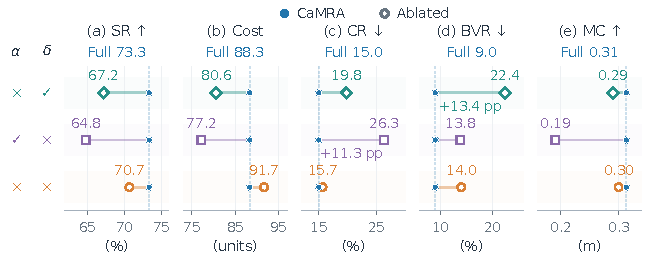
\includegraphics[width=\columnwidth]{../../images/1114/ablation_horizontal.pdf}
\caption{Effects of removing the cost margin $\alpha$ and geometric margin
$\delta$ at the common reference budget. Changes between variants are indicated
by connecting lines.}
\label{fig:ablation_margins}
\end{figure}

To assess margin sensitivity beyond component removal, the high-level networks
are retrained for each of 16 combinations
of $\alpha\in\{0,0.09,0.18,0.27\}$ and
$\delta\in\{0,0.06,0.12,0.18\}$ m, with the frozen tracker, training
budget, and 900-trial evaluation protocol retained. The four zero/calibrated combinations
match Table~\ref{tab:ablation_draft}. With both margins increased to $(0.27,0.18)$,
CR and BVR are reduced to 13.3\% and 6.7\%, but SR is lowered to 68.0\% and
cost is raised to 95.0 a.u. A more conservative trade-off is thus observed as the
margins are increased.
Calibration is performed before the sweep and is not retuned to maximize these
results.

\subsection{Budget Selection and Performance Trade-offs}
\label{sec:budget_sensitivity}
With policy parameters and margins fixed, the effect of initial budget on
navigation performance is evaluated. Budget selection is performed on a separate
rollout set, while Fig.~\ref{fig:budget_draft} reports performance on the final
evaluation set. Since RA is not conditioned on budget, the same trajectories are
evaluated at each threshold, and only its BVR changes. Under the criteria
SR $\geq60\%$, CR $\leq20\%$, and BVR $\leq15\%$, the smallest tested budget
ratios satisfying all three criteria on the final response curves are $0.90$
for CaMRA, $0.96$ for RC-PPO, and $1.12$ for RA. The same evaluation criteria
are therefore met at a lower tested budget with CaMRA.
\begin{figure}[!htbp]
\centering
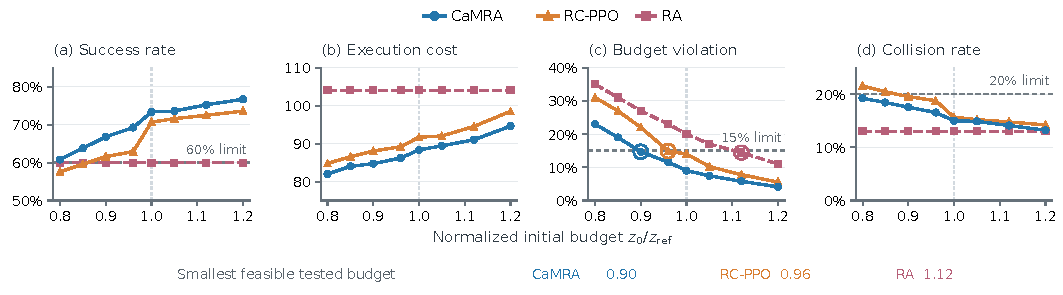
\includegraphics[width=\columnwidth]{../../images/1114/budget_sweep_horizontal.pdf}
\caption{Budget-response curves averaged equally across scenarios. Acceptance
thresholds are indicated by dashed lines; the smallest tested budgets satisfying
all three criteria are marked by outlined points. Results at the reference budget match
Table~\ref{tab:main_results}.}
\label{fig:budget_draft}
\end{figure}

\subsection{Robustness to Execution Perturbations}
\label{sec:execution_robustness}
With the policy and margins fixed, performance is evaluated under execution
conditions that differ from those used for calibration. Each profile's deviation
from the nominal condition is increased by 25\%: the minimum friction is
0.4875, the maximum delay is 0.125 s, and the maximum
velocity-noise standard deviation is 0.05 m/s. Across 900 independent
trials (60 per profile and scene), SR is
$65.0\%$ and BVR $16.0\%$ for CaMRA versus SR $58.0\%$ and BVR $24.0\%$ for
uncalibrated RC-PPO. The corresponding CR values are 22.0\% and 27.0\%, costs
are 96.8 and 102.4 a.u., and MC values are 0.26 and 0.24 m. No policy or margin
is refitted for this stress test. Under the tested perturbations, higher success
and lower collision and budget-violation rates are obtained with CaMRA than with
uncalibrated RC-PPO.

\subsection{Physical-Robot Deployment and Failure Analysis}
\label{sec:hardware_deployment}
A Unitree Go2 is used in two cluttered indoor settings. An obstacle-filled
corridor is shown in Fig.~\ref{fig:hardware_sequences}(a), where collision
avoidance during traversal is examined. A chair arrangement with multiple
available routes is shown in Fig.~\ref{fig:hardware_sequences}(b), where low-cost
route selection under obstacle constraints is examined.

\begin{figure}[!htbp]
\centering
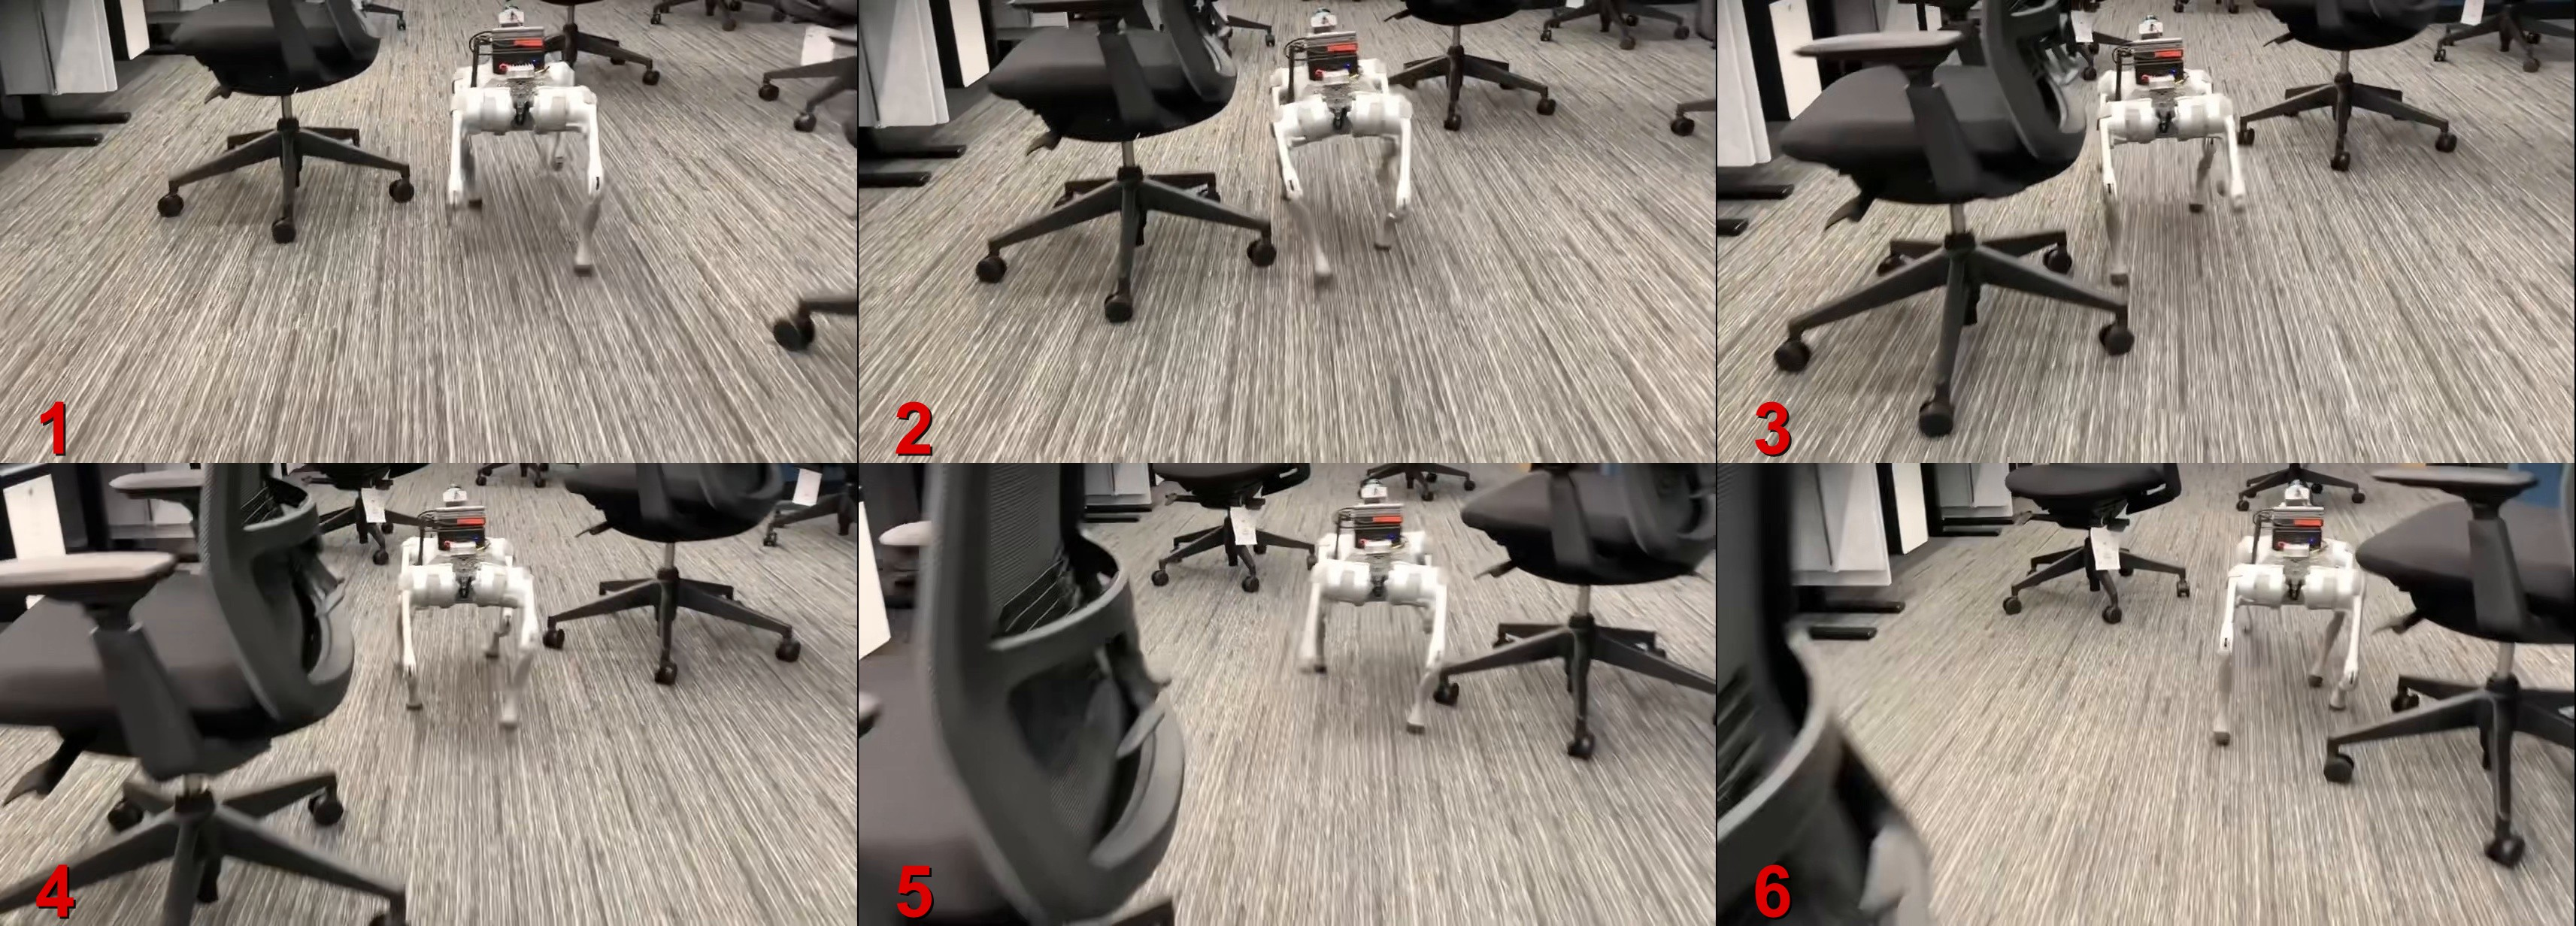
\includegraphics[width=\columnwidth]{../../images/1114/office_sequence_candidate_A_numbered.jpg}
\par\smallskip
{\footnotesize (a) Obstacle avoidance in a cluttered corridor.\par}
\medskip
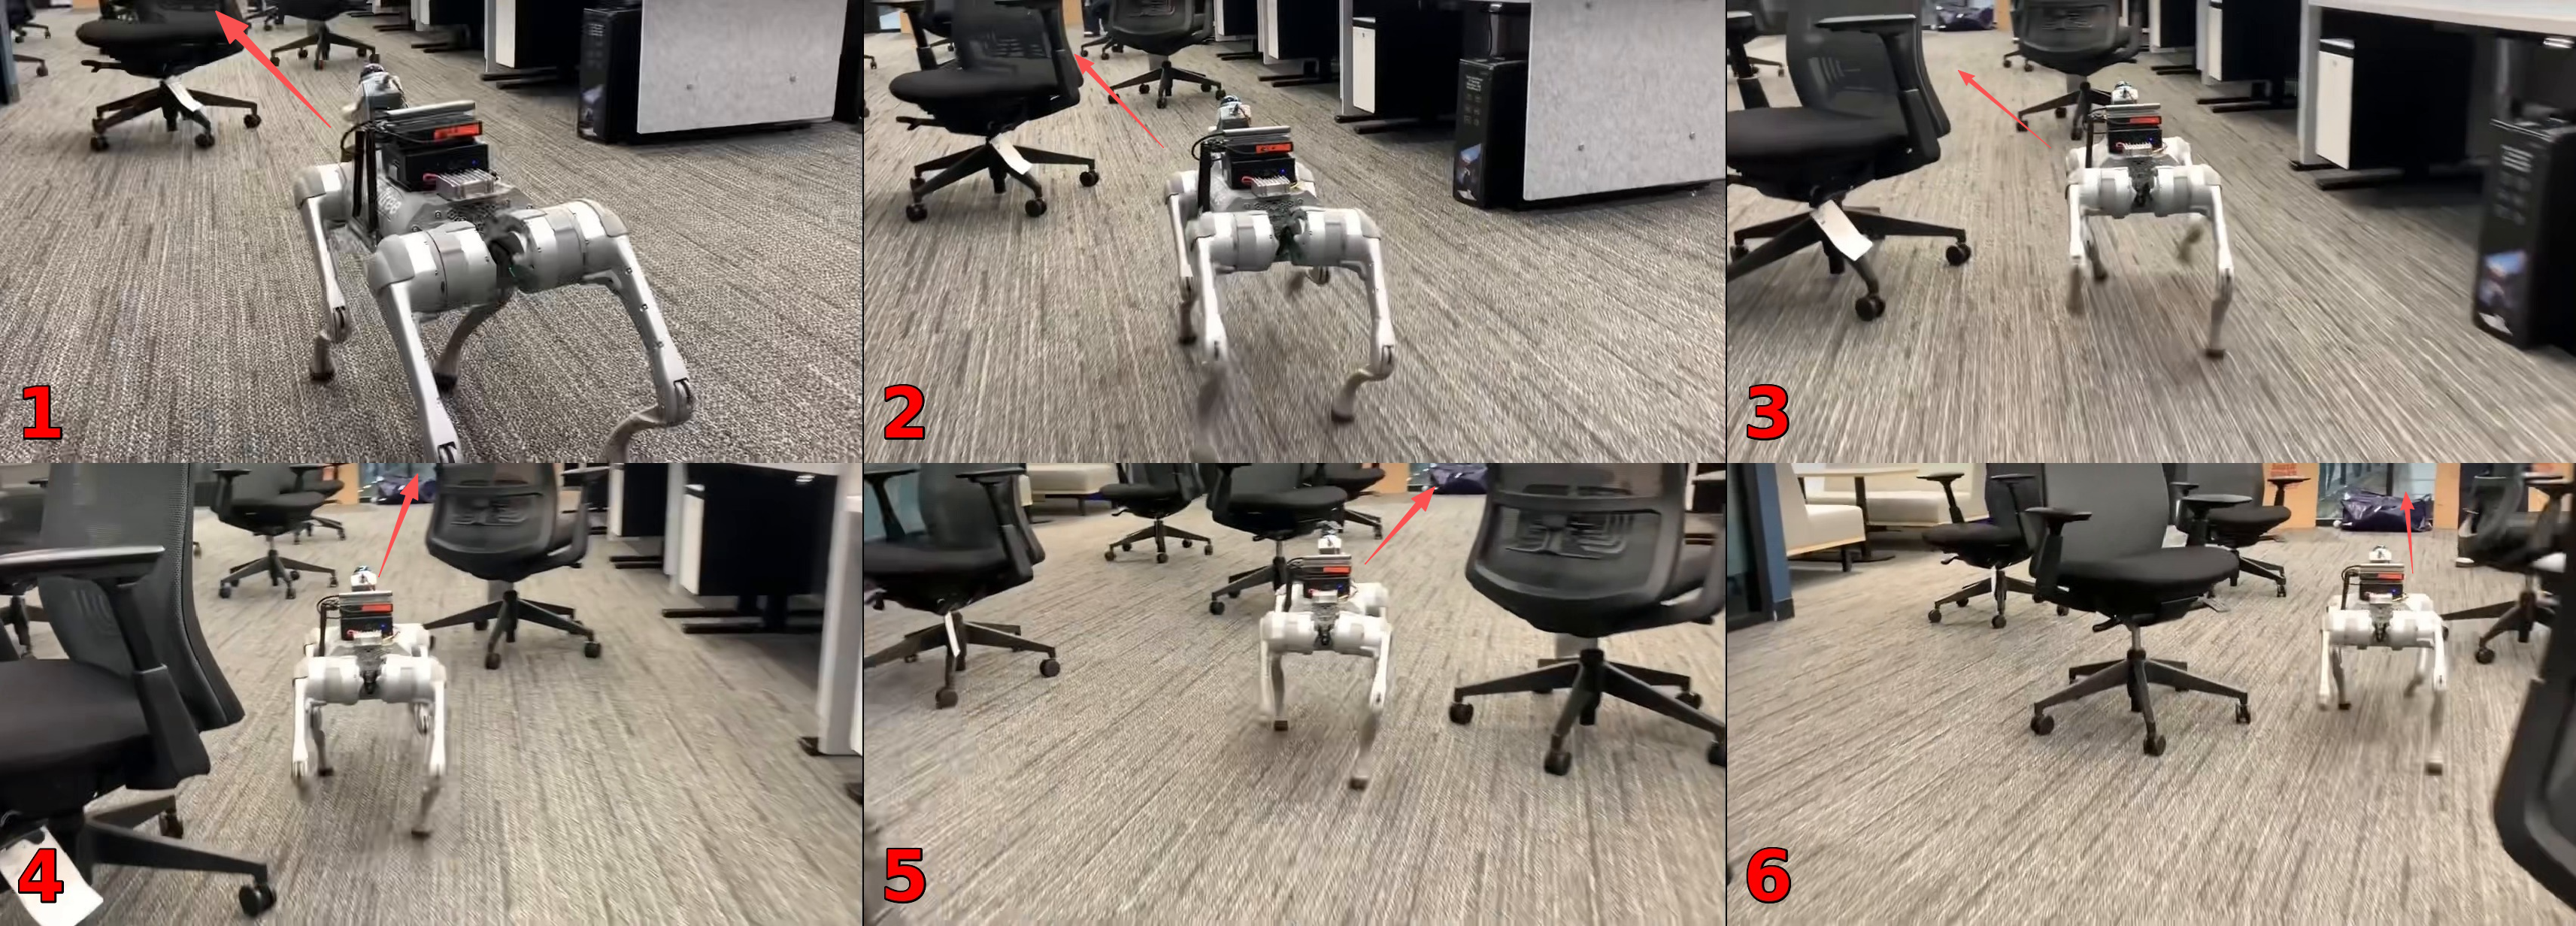
\includegraphics[width=\columnwidth]{../../images/1114/office_shortest_path_sequence_final.png}
\par\smallskip
{\footnotesize (b) Low-cost route selection among chair obstacles.\par}
\caption{Physical deployment of Unitree Go2: (a) corridor traversal with obstacle
avoidance; (b) route selection among multiple passages formed by chairs. Each
panel comprises six successive frames in temporal order; the travel direction
is indicated by red arrows in (b).}
\label{fig:hardware_sequences}
\end{figure}

The representative route is approximately 15 m long and includes a narrow
passage about 0.3 m wider than the robot body. Proprioceptive measurements are
provided by joint encoders and the IMU; navigation observations are obtained from
projected LiDAR ranges and local scan matching.
Policies are executed on an onboard x86-64 CPU with 16 GB RAM, at the same
50 Hz/5 Hz control rates. A 60 s horizon and a budget of 230 a.u. are used for the
15 m task; the tracker, navigation policy, and margins are held fixed.

CaMRA is compared with uncalibrated RC-PPO in Table~\ref{tab:hardware_comparison}
under matched scene conditions, starts, goals, and budget. The same frozen tracker
and navigation inputs are used for both methods; their high-level policies are fixed
throughout evaluation.

\begin{table}[!htbp]
\caption{Hardware performance comparison with 50 trials per method.
Cost is in a.u. and is interpreted jointly with SR.}
\label{tab:hardware_comparison}
\centering
\small
\setlength{\tabcolsep}{3pt}
\renewcommand{\arraystretch}{1.12}
\begin{tabular}{@{}lccccc@{}}
\hline
Method & \shortstack{SR\\(\%) $\uparrow$} & Cost & \shortstack{CR\\(\%) $\downarrow$} & \shortstack{BVR\\(\%) $\downarrow$} & \shortstack{MC\\(m) $\uparrow$}\\
\hline
\rowcolor{methodblue!9}
\textbf{CaMRA} & \textbf{70.0} & 182.0 & \textbf{16.0} & \textbf{14.0} & \textbf{0.09}\\
RC-PPO & 64.0 & \textbf{176.0} & 20.0 & 22.0 & 0.07\\
\hline
\end{tabular}
\end{table}

Success counts are $35/50$ for CaMRA and $32/50$ for RC-PPO. Both methods
have three localization aborts; the remaining failures comprise four timeouts and eight contacts
for CaMRA, versus five timeouts and ten contacts for RC-PPO. BVR decreases
from 22.0\% to 14.0\%, while mean cost increases from 176.0 to 182.0 a.u.
These results indicate a clearance--cost trade-off: shorter routes and
earlier failures can lower mean cost without reducing its upper tail.
All terminal outcomes are included in Cost and MC. Results are reported separately
from the planar benchmark because the route, horizon, and footprint differ.

\section{Conclusion}
The deployment of minimum-cost reach-avoid navigation on quadrupedal robots is
addressed through hierarchical control and execution calibration in CaMRA. The
difficulty of jointly learning locomotion and navigation is mitigated by assigning
motion stabilization to a frozen low-level controller and navigation decisions to
a high-level policy. Remaining discrepancies between nominal and executed behavior
are accounted for through separate cost and geometric margins. The reported
evaluations illustrate the effects of these corrections on budget compliance,
obstacle clearance, and goal reachability.
Building on the current geometric navigation formulation, future work will be
directed toward semantic task understanding and a stochastic formulation in which
execution uncertainty can be incorporated into formal reach-avoid and cost
guarantees.

% Activate balancing within the first column of the reference page.
\IEEEtriggeratref{1}
\IEEEtriggercmd{\balance}
\bibliographystyle{IEEEtran}
\bibliography{references}

\end{document}
